The generation of the Graphs and the Monte Carlo Simulation are implemented
in C, all needed random numbers are generated by the GSL \cite{GSL}
implementation of the \emph{Mersenne Twister} \cite{Matsumoto1998} and
the generated data is evaluated via Python scripts.
All source code is available at \url{https://github.com/surt91/IsingFerromagnet}.\\

For evaluation the Monte Carlo simulation is run until the system
is equilibrated after \(t_{eq}\) sweeps. Then the simulation continues
and the magnetization per site \(m=\frac{1}{N}\sum_i s_i\) and energy
per site \(E=\frac{1}{N}\hat H\) are calculated and saved for every
\(2\tau\) sweeps. Where \(\tau\) denotes the \emph{autocorrelation time}
(see also \ref{ssec:eqtime}). The used values for different system sizes
are listed in tab. \ref{tab:tauAndTeq} in numbers of sweeps. Note that
the \(t_{eq}\) values are generously rounded up to be on the safe side
and the \(\tau\) values are determined as the maximum \(\tau\) over all
simulated temperatures and disorder parameters \(\tau = \underset{T,\sigma}{\max} \{\tau_{T,\sigma}\}\)
and rounded up to the next integer.
\begin{table}[htbp]
    \center
    \begin{tabular}{l r r r r r}
        \toprule
        \(L\)    & 16 &  32 &  64 & 128 & 256\\
        \midrule
        \(\tau\) &  3 &   5 &   7 &  12 &  16\\
        \(t_{eq}\) & 40 & 100 & 100 & 200 & 600\\
        \bottomrule
    \end{tabular}
    \caption{Autocorrelation Times $\tau$ and Equilibration Times $t_{eq}$}
    \label{tab:tauAndTeq}
\end{table}\\
For every observable \(O\) the expected value \(\avg{O}\) is determined
as the mean of \(N_{\mathrm{measure}}=10000\) measurements for \(L=16,32\)
or \(N_{\mathrm{measure}}=5000\) for \(L=64,128\). The number of
calculated sweeps totals to
\[N_{\mathrm{sweeps}}=t_{eq}+2\tau N_{\mathrm{measure}}\]
The expected values \(\avg{O}\) for \(100\) different random proximity
graphs with the same disorder parameter \(\sigma\) are then averaged to
\(\overline{\avg{O}}\). Not only the seed to generate the new random
realization of the proximity graph gets changed, but also the seed for
the random numbers used in the Monte Carlo simulation and during the
generation of the random start configuration of the spins.\\
The errors \(\Delta \overline{\avg{O}}\) are estimated by bootstrapping
\cite{Bootstrap} with 200 bootstrap samples if not noted otherwise.
Note that while \(\Delta \avg{O}\) is dependend on \(\tau\) \cite[p. 151]{Katzgraber2011}
\(\Delta \overline{\avg{O}}\) is not directly, because it is averaged
over different realizations of the random proximity graph, which are
surely uncorrelated.
Because every error mentioned in this thesis is of this type, it is not
necessary to determine \(\tau\) for each observable. Therefore a good
error estimate can be achieved by simple bootstrapping. Though one has
to simulate enough uncorrelated states for each realization, to keep
the \(\Delta \overline{\avg{O}}\) small.

\subsection{Short Analysis of the Autocorrelation Time  $\tau$}
    % Sollte das hier rein?
    Before the results are presented, a short analysis of the
    autocorrelation time \(\tau\) is given, to illustrate the benefits
    of the used Wolff cluster algorithm.\\
    In \ref{fig:autocorr}\subref{fig:autocorr:temperatures}
    the autocorrelation time for the magnetization per site \(m\) at \(\sigma=0\) is plotted.
    \begin{figure}[htbp]
        \centering
        \subfigure[in dependence on the temperature $T$][]
        {
            \label{fig:autocorr:temperatures}
            \includegraphics[width=0.45\textwidth]{plots/autocorrT}
        }
        \subfigure[in dependence on the system size $L$][]
        {
            \label{fig:autocorr:powerLaw}
            \includegraphics[width=0.45\textwidth]{plots/autocorrL}
        }
        \caption[The autocorrelation time $\tau$]
        {
            Dependece of the autocorrelation time $\tau$ on
            \subref{fig:autocorr:temperatures} the temperature $T$ for
                $\sigma=0$ and
            \subref{fig:autocorr:powerLaw} the system size $L$ (errorbars
                are the standard error determined by bootstrapping)
        }
        \label{fig:autocorr}
    \end{figure}
    The plateau at low temperatures is easy to understand considering the
    effects of the Wolff algorithm. At low temperatures it flips nearly every
    spin in every step, thus the correlation drops to zero after one sweep.
    Alternatively the parallel tempering algorithm swaps spin configurations
    with possibly different signs, thus having the same effect.
    Also note that the maximum of \(\tau\) is not at \(T_c\) but at a higher
    temperature. The cause is probably the effectiveness of the Wolff cluster
    algorithm at \(T_c\).
    Obviously the autocorrelation time \(\tau\) increases with the system
    size. In fact it obeys a power law, which is the expected behaivior of
    a dynamical critical exponent \(z\) as mentioned in section \ref{ssec:eqtime}.
    In fig. \ref{fig:autocorr}\subref{fig:autocorr:powerLaw} \(\tau\) is plotted
    over \(L\) and the dynamical exponent \(z'\) is determined as \(z'=0.64(2)\).
    This exponent is much higher than the one of Wolff cluster
    algorithm at criticality, which is \(z=0.25\)\cite{NewmanBarkema1999}.
    So it represents the dynamical exponent for parallel tempering with
    Metropolis above criticality and thus is not exactly a critical exponent.
    Nevertheless it is interesting, that it obeys a power law just the same.
    Anyhow it is a proof for the effectiveness of the Wolff cluster algorithm
    at criticality.

\subsection{Finite Size Effects}
\label{ssec:finitesize}
    The aim of this thesis is to find the critical temperature \(T_c\)
    of the disordered Ising model in dependence of the disorder parameter
    \(\sigma\). At \(T_c\) the mean absolute magnetization \(\avg{|m|}\) of
    the system will jump and the susceptibility
    \(\chi = \frac{N}{T}\brac{\avg{m^2}-\avg{m}^2}\)
    will diverge. In fig. \ref{fig:smeared_out}\subref{sfig:smeared_out:meanM_L}
    it is easy to see that the jump of \(\avg{|m|}\)
    occurs at lower temperatures \(T\) for higher
    disorder parameters \(\sigma\) (here with a RNG).
    \begin{figure}[htbp]
        \centering
        \subfigure[Dependence of the phase transition on $\sigma$][]
        {
            \label{sfig:smeared_out:meanM_L}
            \includegraphics[width=0.45\textwidth]{plots/Mean_M_L_128}
        }
        \subfigure[Example for finite size effects][]
        {
            \label{sfig:smeared_out:meanM}
            \includegraphics[width=0.45\textwidth]{plots/meanM}
        }
        \caption[Phase Transition and Finite Size Effects]
        {
            \subref{sfig:smeared_out:meanM_L}: Effects of the disorder
            parameter $\sigma$ on the phase transition
            for an underlying RNG with $L=128$.\\
            \subref{sfig:smeared_out:meanM}: Effects of different system
            sizes at \(\sigma = 0\). Dotted lines are guides to the eye.
        }
        \label{fig:smeared_out}
    \end{figure}\\
    But in the shown plots there occurs no real jump, but a continuous
    decline. The jump is only present in infinite systems, hence no
    computer simulation will show the exact behavior in the
    thermodynamic limit. It will always show some \emph{finte size effects}.
    These finite size effects cause a "smearing out" of the phase
    transition. This is stronger for smaller system sizes, as is visible
    in fig. \ref{fig:smeared_out}\subref{sfig:smeared_out:meanM}\footnote{See the appendix \ref{appendix:finiteSizeEffects} for a similar figure for the specific heat.}.
    Clearly the \(L=16\) curve is much less steep than the \(L=128\) curve.\\
    Despite of this one can obtain \(T_c\) by finite size scaling
    methods \cite[S. ??]{NewmanBarkema1999} which also yield the critical
    exponents.
    Studies on random lattices with\cite{Lima2000} and without\cite{Janke1994}
    varying coupling constants \(J\) suggest, that the
    critical exponents should not be influenced by the disorder parameter
    \(\sigma\). So they will be used for consistency cross checking and
    comparison with the known exact values \cite[S. 59]{Pelissetto2002}.\\
    % Ausfuehrlichere Herleitung der Skalentheorie, Skalenanalyse
    For a more in depth look at finite size scaling, \cite{Norrenbrock2011}
    offers an explanation.
    It is known, that for large \(L\) near the critical temperature the
    equations \eqref{eq:fsscaling:m}, \eqref{eq:fsscaling:chi} and
    \eqref{eq:fsscaling:g} apply.
    \begin{align}
        \label{eq:fsscaling:m}
        \avg{m_L} &= L^\frac{\beta}{\nu} \tilde{M}\brac{L^\frac{1}{\nu}\brac{T-T_c}}\\
        \label{eq:fsscaling:chi}
        \chi_L    &= L^\frac{\gamma}{\nu} \tilde{C}\brac{L^\frac{1}{\nu}\brac{T-T_c}}\\
        \label{eq:fsscaling:g}
        g          &= \frac{3}{2}\brac{1-\frac{\avg{m^4}}{3\avg{m^2}^2}} \propto \tilde{G}\brac{L^\frac{1}{\nu}\brac{T-T_c}}
    \end{align}
    Where \(g\) from eq. \eqref{eq:fsscaling:g} is a normalized
    Binder cumulant \cite{Binder1981} and \(\tilde{M}, \tilde{C}\) and \(\tilde{G}\)
    are unknown scaling functions. To find the exponents
    \(\beta, \gamma, \nu\) and the critical temperature \(T_c\), one
    varies them until the measured values of the observables collapse on
    one curve. Like the obersables from fig. \ref{fig:gettingCrit}\subref{sfig:gettingCrit:binder_fit_s_0}
    collapse in fig. \ref{fig:gettingCrit}\subref{sfig:gettingCrit:collapse_s_0}%\footnote{Examples for a collapse to determine the other critical exponents are in appendix \ref{appendix:finiteSizeScaling}}.
    Note that \(L=16\) is not used for the collapse, because it is a
    rather small value. Eq. \eqref{eq:fsscaling:m}-\eqref{eq:fsscaling:g}
    are approximations for big \(L\). For small \(L\) one needs some
    \emph{corrections to scaling} terms, which are not considered here.\\
    To accomplish the collapse in an semi-automatic and reproduceable
    way with an error estimate, the program
    \texttt{autoscale.py} \cite{autoscale2009} is used.
    \begin{figure}[htbp]
        \centering
        \subfigure[Example of a Binder cumulant to determine the critical temperature][]
        {
            \label{sfig:gettingCrit:binder_fit_s_0}
            \includegraphics[width=0.47\textwidth]{plots/binder_fit_s_0}
        }
        \subfigure[Example of a datacollapse to determine critical exponents][]
        {
            \label{sfig:gettingCrit:collapse_s_0}
            \includegraphics[width=0.47\textwidth]{plots/collapse_s_0}
        }
        \caption[Examples of determining critical temperature and exponents]
        {
            The Binder cumulant \(g\) of an square lattice Ising model
            (\(\sigma=0\))\\
            \subref{sfig:gettingCrit:binder_fit_s_0} interpolated
                with cubic splines (the errorbars are too small to see)\\
            \subref{sfig:gettingCrit:collapse_s_0} collapsed by finite
                size scaling
        }
        \label{fig:gettingCrit}
    \end{figure}\\
    Though if one is just interested in the critical Temperature, an
    easier approach is to find the intersections of the Binder cumulants
    \(g\) of different system sizes \(L\) because they are intersecting
    at \(T_c\) \cite{Binder1981}.
    Because the magnetization \(m\) is only measured for discrete values
    of \(T\), \(g\) is also only known for these discrete values and the
    analytical course of the curve is not known, and hence has
    to be interpolated to find the intersection. Therefore a \emph{cubic spline}
    interpolation\footnote{created using the \texttt{scipy.interpolate} tools \cite{scipy2001}}
    is calculated for the measured points.
    Cubic spline interpolation is a piece wise fitting of polynoms of
    degree three which are joined under the condition to be at least two
    times continuously differentiable. This interpolation type has the
    advantage, that it is only influenced by local points so that the
    plateaus at low and high \(T\) do not influence the interpolation in
    the vicinity of \(T_c\) -- in contrast to e.g. an polynom fit of
    degree 4, which has to be restricted to the vincinity of \(T_c\) to
    yield meaningful results.
    As an example take fig. \ref{fig:gettingCrit}\subref{sfig:gettingCrit:binder_fit_s_0}.
    Here such interpolations are plotted for \(\sigma=0\) and are
    intersecting at \(\approx 2.27\).
    To determine \(T_c\), the intersections\footnote{found using the \texttt{scipy.optimize} tools \cite{scipy2001}}
    are averaged and the standard error is calculated. In this case one
    gets \(T_c = 2.2689(2)\), which is in good agreement with the
    exact solution from eq. \eqref{eq:exactTc} \cite{Onsager1944}.
    \begin{equation}
        T_c = 2J/\ln(1+\sqrt 2) = 2.2691...
        \label{eq:exactTc}
    \end{equation}
    This test suggests, that measuring \(T_c\) this way is yields
    adequat results and the interpolation does not lead to major
    deviations.

\subsection{Critical Temperature}
\label{ssec:binderIntersections}
    The evaluation of the Binder cumulant's intersections, yields the
    critical temperatures \(T_c\).
    In this section these \(T_c\) on either the RNG or the GG are
    compared. In the following figures, the RNG will always be on the
    left side and the GG on the right side.
    In fig. \ref{fig:Tc} \(T_c\) is plotted over \(\sigma\).
    \begin{figure}[htbp]
        \centering
        \subfigure[][]
        {
            \label{sfig:Tc:RNG}
            \includegraphics[width=0.45\textwidth]{plots/RNG_Tc}
        }
        \subfigure[][]
        {
            \label{sfig:Tc:GG}
            \includegraphics[width=0.45\textwidth]{plots/GG_Tc}
        }
        \caption[Critical Temperature over different disorder parameters]
        {
            Critical temperatures \(T_c\) over different
            disorder parameters \(\sigma\) for
            \subref{sfig:Tc:RNG} the RNG and
            \subref{sfig:Tc:GG} the GG.\\
        }
        \label{fig:Tc}
    \end{figure}\\
    One sees that the RNG on the left has generally a lower critical
    temperature than the GG. Also \(T_c\) of the RNG decreases
    monotonically while \(T_c\) of the GG rises at first. Naively one would
    expect, that while changing the displacement of the nodes monotonically,
    the properties of the system will also change monotonically. The
    maximum at \(\sigma \approx 0.15\) on the GG will be discussed later.
    For big \(\sigma\) the displaced nodes approach the limit of randomly
    distributed nodes, hence \(T_c\) is independent of \(\sigma\) for
    \(\sigma \gg 1\).\\
    Another strange property is the jump from \(\sigma = 0\) to \(\sigma > 0\)
    of \(T_c\) on the GG. To understand that, one has to
    consider the influence of the graph properties on the critical
    temperature.\\
    One basic property of a graph is its degree \(K\) -- sometimes
    called \emph{coordination number} -- is defined as the mean count of
    neighbors per node
    \begin{equation}
        K = \frac{\sum_{\avg{i,j}} 1}{\sum_{i} 1}
        \label{eq:degree}
    \end{equation}
    It is known, that the degree has an impact on the critical Temperature.
    For example the Honeycomb lattice is of degree \(K=3\)
    and there exists an analytic solution \cite{Wannier1945}.
    Its critical temperature is determined by eq. \eqref{eq:exactHCTc}.
    \begin{equation}
        \cosh\brac{\frac{J}{T_c}}=2 \overset{J=1}{\Longrightarrow} T_c \approx 1.52
        \label{eq:exactHCTc}
    \end{equation}
    This is lower than for the square lattice with degree 4.\\
    If one plots the degree of the graphs at different \(\sigma\) like
    in fig. \ref{fig:Tc_deg}\subref{sfig:deg:RNG}\subref{sfig:deg:GG},
    one recognizes, that \(T_c\) and \(K\) are evidently correlated.
    It seems reasonable to normalize \(T_c\) by the degree of the underlying
    graph. This is done in fig \ref{fig:Tc_deg}\subref{sfig:Tc_norm_deg:RNG}\subref{sfig:Tc_norm_deg:GG}.
    Indeed the normalization eliminates the jump and reduces the
    slope of the rising on the GG. Hence it reduces differences
    between the RNG and the GG.
    \begin{figure}[htbp]
        \centering
        \subfigure[][]
        {
            \label{sfig:deg:RNG}
            \includegraphics[width=0.45\textwidth]{plots/RNG_deg}
        }
        \subfigure[][]
        {
            \label{sfig:deg:GG}
            \includegraphics[width=0.45\textwidth]{plots/GG_deg}
        }

        \subfigure[][]
        {
            \label{sfig:Tc_norm_deg:RNG}
            \includegraphics[width=0.45\textwidth]{plots/RNG_Tc_norm_deg}
        }
        \subfigure[][]
        {
            \label{sfig:Tc_norm_deg:GG}
            \includegraphics[width=0.45\textwidth]{plots/GG_Tc_norm_deg}
        }

        \caption[Critical Temperature normalized by Degree of the Graph]
        {
            Top: Degree \(K\) of graph over different
            disorder parameters \(\sigma\) for
            \subref{sfig:deg:RNG} the RNG and
            \subref{sfig:deg:GG} the GG.\\
            Bottom: Critical temperatures normalized by degree over different
            disorder parameters for
            \subref{sfig:Tc_norm_deg:RNG} the RNG and
            \subref{sfig:Tc_norm_deg:GG} the GG.
        }
        \label{fig:Tc_deg}
    \end{figure}\\
    To understand the jump of \(T_c\), it seems to be sufficient to
    understand the jump of \(K\), which is easily explained
    by the definition of the GG and its aftereffects for
    the transition from \(\sigma = 0\). Visible in fig. \ref{fig:GG_sigma}\subref{sfig:GG_sigma:0.00}\subref{sfig:GG_sigma:0.01}
    a small change of \(\sigma\) causes many new edges to arise\footnote{See also \url{http://www.youtube.com/watch?v=PcVZ2pG11GI} for an animation.}.
    To fully understand this, take four nodes forming a square. The edge
    across does not exist, because the other two nodes are on the edge
    of the lune. Moving one node slightly into the square, causes the lune
    to get smaller, hence no other nodes are inside or on the edge of
    the lune anymore and the edge appears.\\
    Further the increase of \(T_c\) on the GG can be made plausible.
    Though it is not removed by the normalization, it is reduced. Also
    the maximum of the \(K\) is at the same \(\sigma\), as the maximum
    of \(T_c\). So while displacing the nodes, there arise more edges
    than edges are vanishing until \(\sigma \approx 0.15\) is reached.
    Then more edges disappear, than appear at further displacement. This
    is not an obvious effect, but can be seen in fig. \ref{fig:GG_sigma}\subref{sfig:GG_sigma:0.09}\subref{sfig:GG_sigma:0.15}\subref{sfig:GG_sigma:0.21}
    \begin{figure}[htbp]
        \subfigure[][$\sigma = 0.00$]
        {
            \label{sfig:GG_sigma:0.00}
            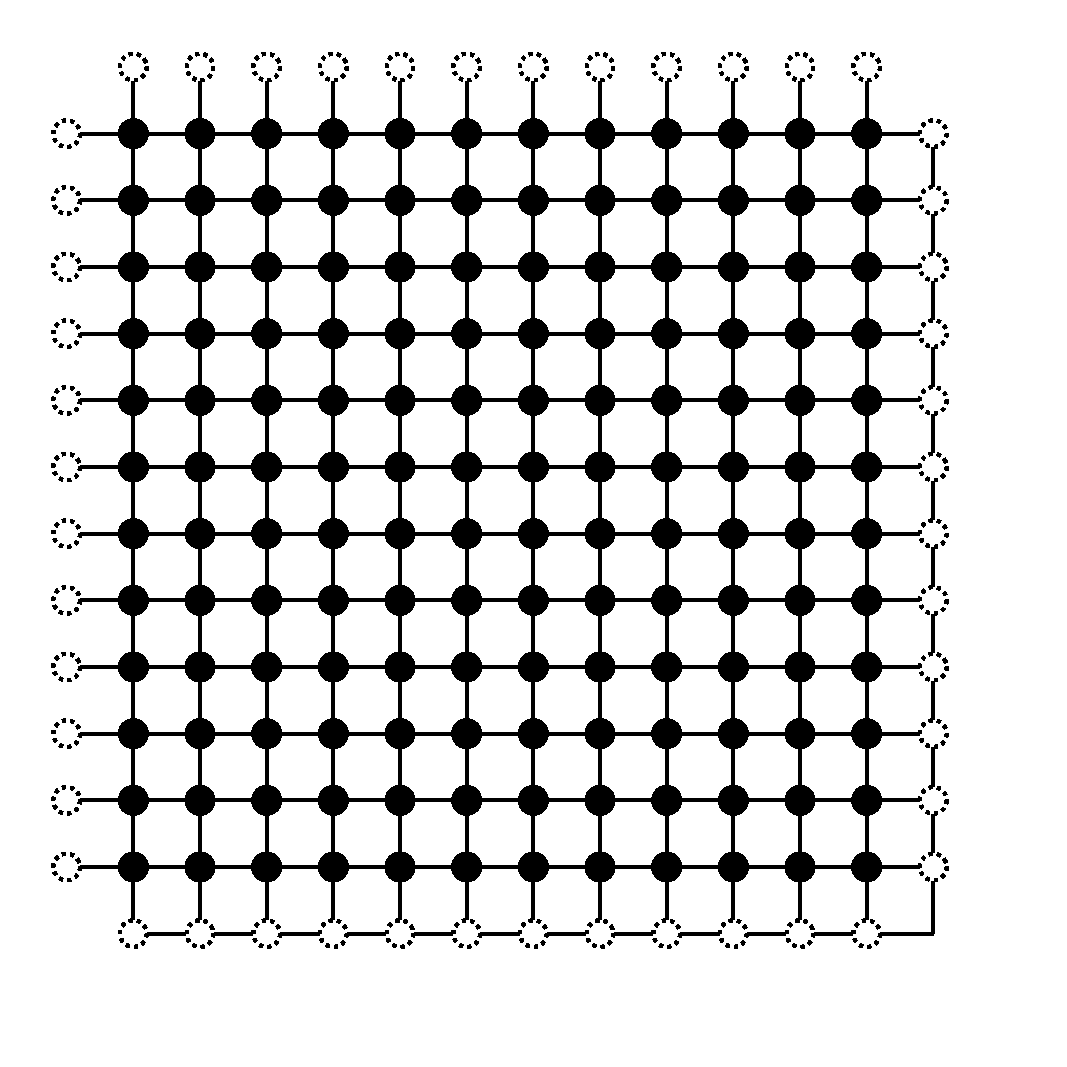
\includegraphics[width=0.30\textwidth]{images/GG/sigma_e0}
        }
        \subfigure[][$\sigma = 0.01$]
        {
            \label{sfig:GG_sigma:0.01}
            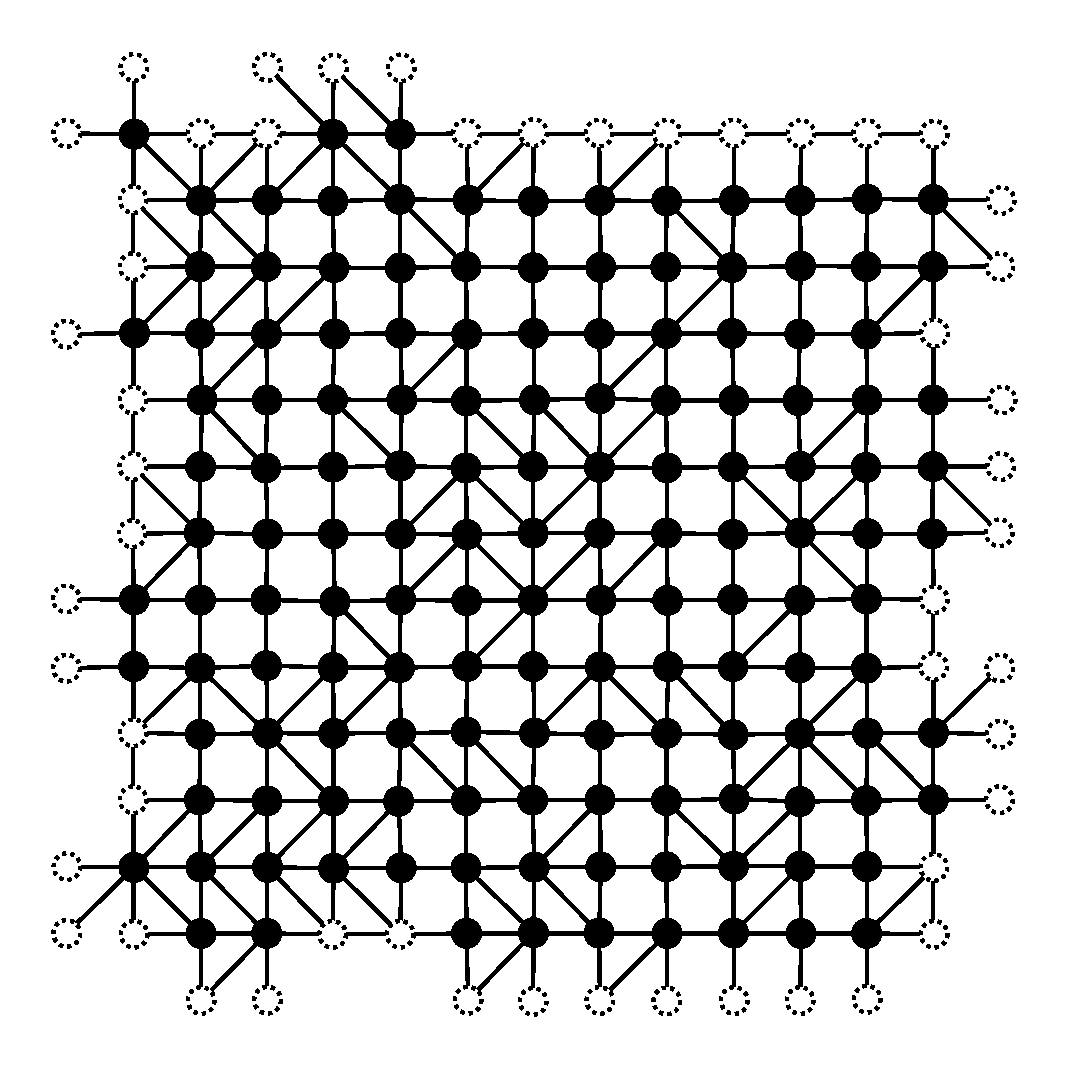
\includegraphics[width=0.30\textwidth]{images/GG/sigma_g0}
        }

        \subfigure[][$\sigma = 0.09$]
        {
            \label{sfig:GG_sigma:0.09}
            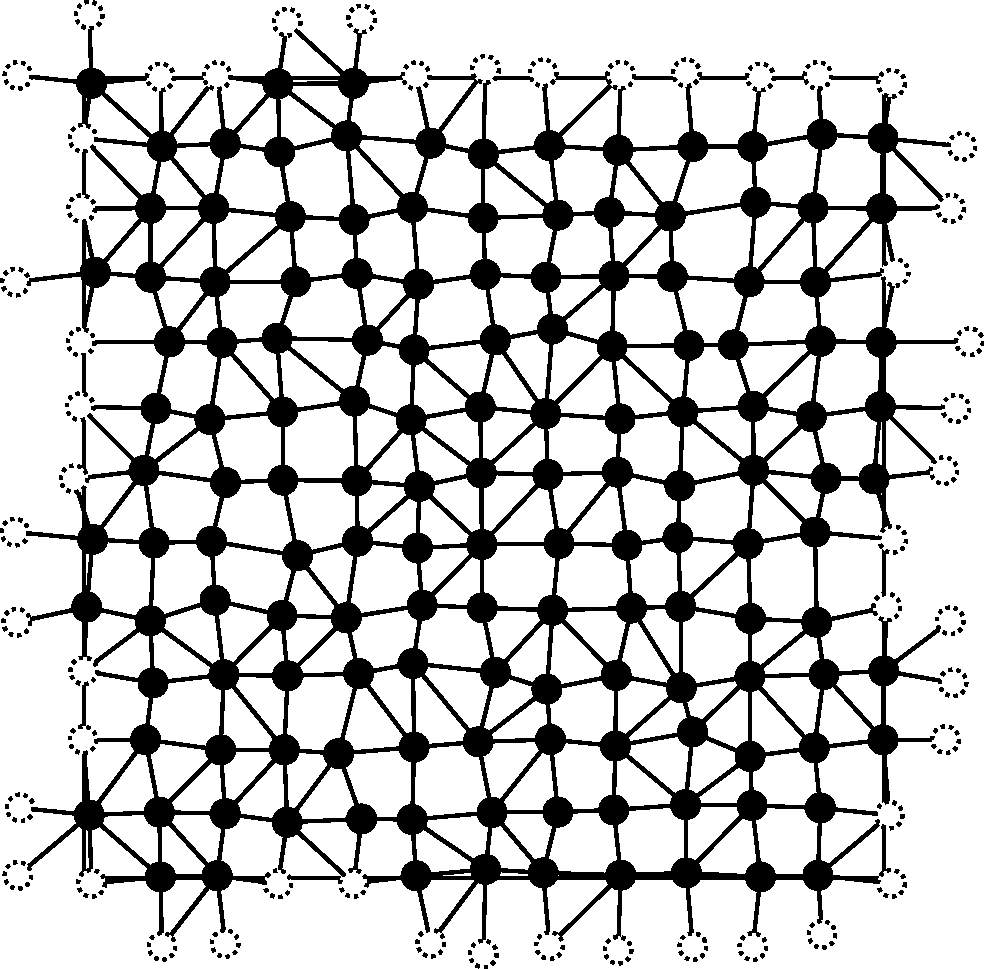
\includegraphics[width=0.30\textwidth]{images/GG/out009}
        }
        \subfigure[][$\sigma = 0.15$]
        {
            \label{sfig:GG_sigma:0.15}
            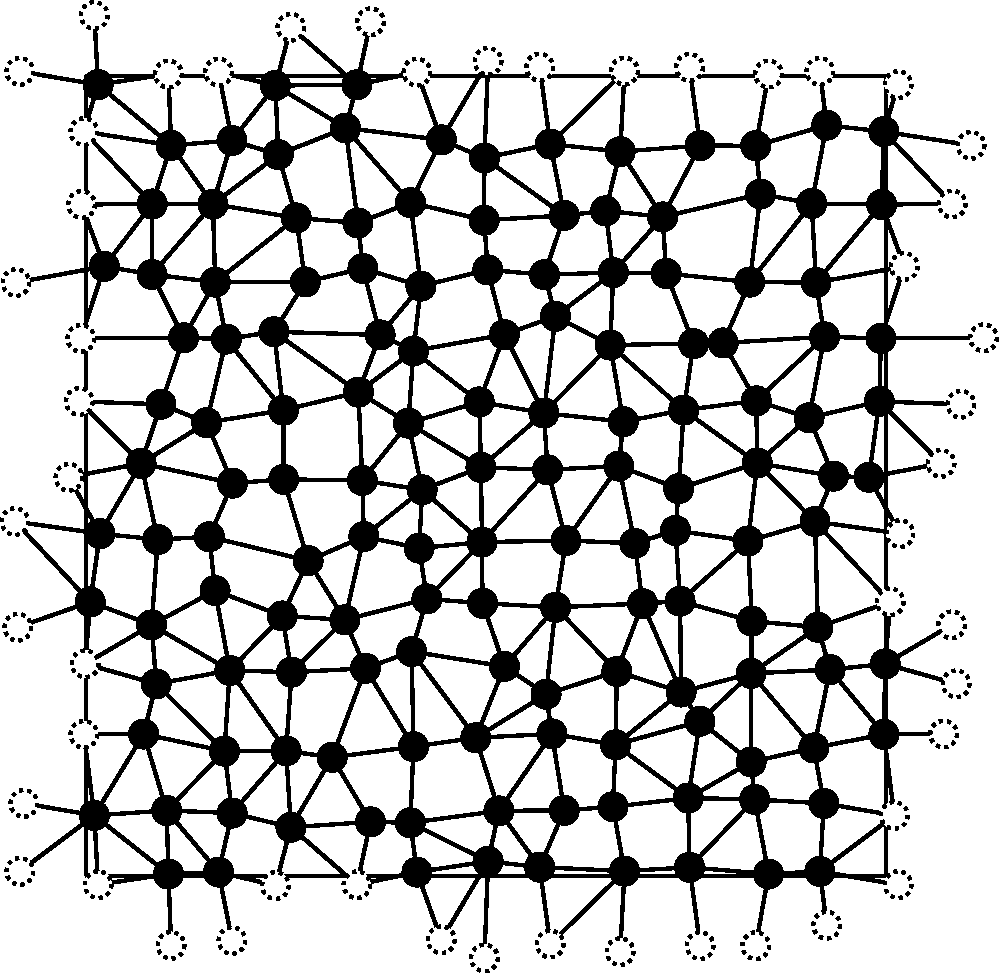
\includegraphics[width=0.30\textwidth]{images/GG/out015}
        }
        \subfigure[][$\sigma = 0.21$]
        {
            \label{sfig:GG_sigma:0.21}
            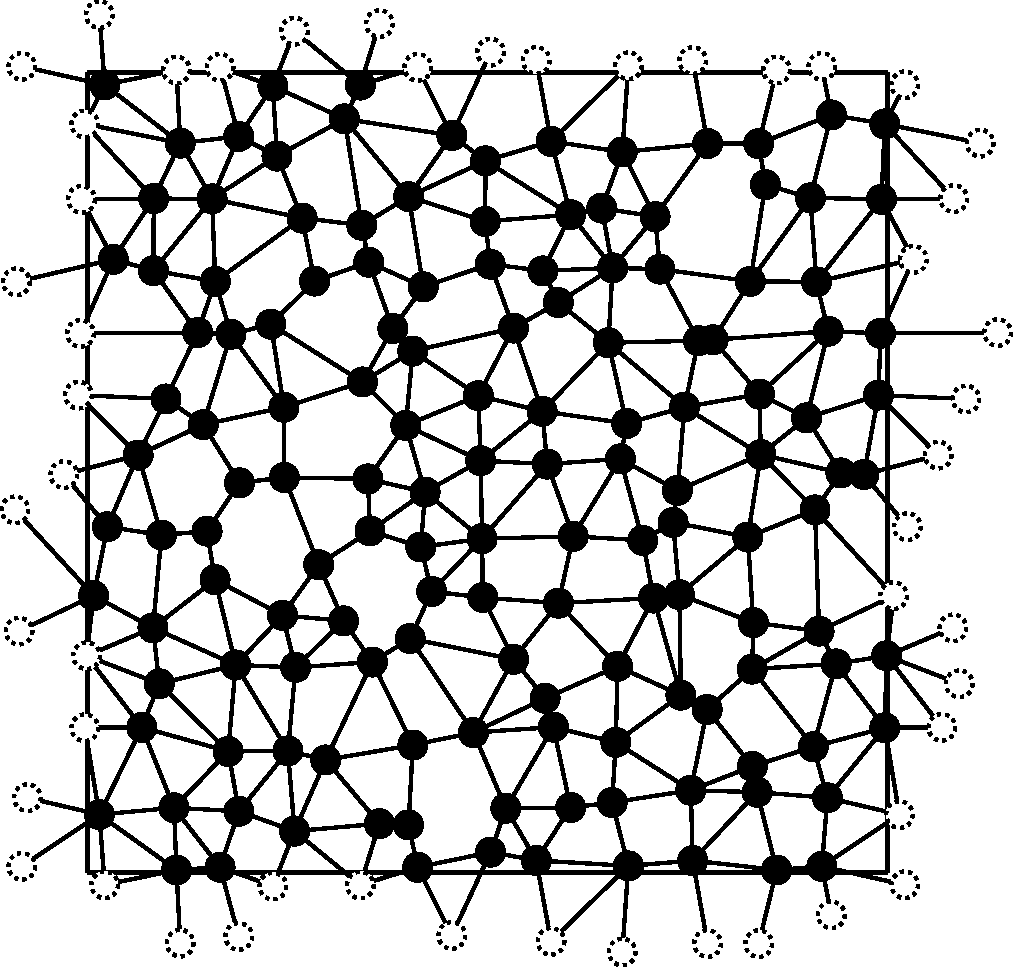
\includegraphics[width=0.30\textwidth]{images/GG/out021}
        }

        \caption[Anomaly of the GG for small $\sigma$]
        {
            GG with periodic boundary conditions for different \(\sigma = 0\)
        }
        \label{fig:GG_sigma}
    \end{figure}\\
    The explanation for the plateau of the RNG at low \(\sigma\) is similar.
    On the RNG no new edges arise at small displacements of the nodes\footnote{See \ref{appendix:RNGDisplacement} for a graphic.}\footnote{See also \url{http://www.youtube.com/watch?v=rltzi15mTM4} for an animation.}.
    But the degree does not alone influence the behavior of \(T_c\).
    Further \(T_c\) depends on the coupling constant \(J\), which is
    obvious in eq. \eqref{eq:exactTc} and \eqref{eq:exactHCTc}. The
    coupling constant in turn is depending on the length of the edges,
    which changes with \(\sigma\).
    Therefore  in fig. \ref{fig:TcJ}\subref{sfig:sumJ:RNG}\subref{sfig:sumJ:GG}
    the mean sum of the coupling constants to all neighbors \(\avg{\sum_{\avg{i,j}} J_{ij}}\)
    is plotted. This is a number which should combine the dependence on
    the degree and the coupling constant.
    The plots fig \ref{fig:TcJ}\subref{sfig:Tc_normJ:RNG}\subref{sfig:Tc_normJ:GG}
    show that \(\avg{\sum_{\avg{i,j}} J_{ij}}\) is also correlated with \(T_c\).
    \begin{figure}[htbp]
        \centering
        \subfigure[][]
        {
            \label{sfig:sumJ:RNG}
            \includegraphics[width=0.45\textwidth]{plots/RNG_sumJ}
        }
        \subfigure[][]
        {
            \label{sfig:sumJ:GG}
            \includegraphics[width=0.45\textwidth]{plots/GG_sumJ}
        }

        \subfigure[][]
        {
            \label{sfig:Tc_normJ:RNG}
            \includegraphics[width=0.45\textwidth]{plots/RNG_Tc_normJ}
        }
        \subfigure[][]
        {
            \label{sfig:Tc_normJ:GG}
            \includegraphics[width=0.45\textwidth]{plots/GG_Tc_normJ}
        }

        \caption[Critical Temperature normalized by Mean Sum of the Coupling Constants]
        {
            Top: Mean sum of the coupling constants to all
            neighbors over different disorder parameters for
            \subref{sfig:sumJ:RNG} the RNG and
            \subref{sfig:sumJ:GG} the GG.\\
            Bottom: Critical temperatures normalized by mean sum of the
            coupling constants \(\avg{\sum_{\avg{i,j}} J_{ij}}\) over different
            disorder parameters for
            \subref{sfig:Tc_normJ:RNG} the RNG and
            \subref{sfig:Tc_normJ:GG} the GG.
        }
        \label{fig:TcJ}
    \end{figure}\\
    Though the eq. \eqref{eq:exactHCTc} shows, that there does not have
    to be a linear connection between \(J\) and \(T_c\), the best guess
    is a linear connection, because this model is derived from the
    square lattice, where the connection is linear. Therefore, one
    normalizes \(T_c\) with \(\avg{\sum_{\avg{i,j}} J_{ij}}\) as in
    \ref{fig:TcJ}\subref{sfig:Tc_normJ:RNG}\subref{sfig:Tc_normJ:GG}, the
    jump on the GG arises again, but \(T_c\) is now monotonically
    decreasing with increasing disorder parameter \(\sigma\).
    %~ This is a strong hint, that the change of the \(T_c\) with changing
    %~ \(\sigma\) is in some way connected to \(J\) and \(K\) which is an
    %~ expected conclusion.\\
    Moreover the forms of both curves are quite similar, but the
    one for the RNG \ref{fig:TcJ}\subref{sfig:Tc_normJ:RNG}
    is generally lower and spans over a bigger temperature range than
    the curve of the GG \ref{fig:TcJ}\subref{sfig:Tc_normJ:GG}.
    Both graph types have a plateau at \(0 < \sigma < 0.1\). So small
    disorder has little influence on this normalized critical temperature.
    Also both graph types have a steep decline after the plateau before
    they approach an asymptotic limit for \(\sigma \gg 1\)\\\\

\subsection{Critical Exponents}
    A finite size scaling analysis was
    performed to determine the critical exponents \(\beta, \gamma, \nu\)
    using \texttt{autoscale.py} \cite{autoscale2009} and eq. \eqref{eq:fsscaling:m}-\eqref{eq:fsscaling:g}.
    The values for \(\nu\) are yielded by every collapse and are therefore
    averaged over all determined values. Fig. \ref{fig:gettingCrit2}\subref{sfig:gettingCrit:s_0_sus}\subref{sfig:gettingCrit:collapse_s_0_sus}
    show an example collapse for \(\sigma=0\) of the magnetic susceptibility
    \[\chi = \frac{1}{TN}\avg{\avg{m^2} - \avg{m}^2}\]
    This way the exponents \(\gamma\) and \(\nu\) are determined.
    Analogical fig. \ref{fig:gettingCrit2}\subref{sfig:gettingCrit:s_0_meanM}\subref{sfig:gettingCrit:collapse_s_0_meanM}
    shows the collapse for the mean absolute magnetisation per site \(\avg{\abs{m}}\) for \(\sigma=0\),
    to determine the exponents \(\beta\) and \(\nu\).
    Also the collapse of the binder cumulant as mentioned before and shown
    in fig. \ref{fig:gettingCrit}\subref{sfig:gettingCrit:collapse_s_0}
    is used to get a further value of \(\nu\).
    \begin{figure}[htbp]
        \centering
        \subfigure[Susceptibility $\chi$][]
        {
            \label{sfig:gettingCrit:s_0_sus}
            \includegraphics[width=0.47\textwidth]{plots/s_0_sus}
        }
        \subfigure[Finite Size Scaling of the Susceptibility $\chi$][]
        {
            \label{sfig:gettingCrit:collapse_s_0_sus}
            \includegraphics[width=0.47\textwidth]{plots/collapse_s_0_sus}
        }
        \subfigure[Magnetisation $\avg{\abs{m}}$][]
        {
            \label{sfig:gettingCrit:s_0_meanM}
            \includegraphics[width=0.47\textwidth]{plots/s_0_meanM}
        }
        \subfigure[Finite Size Scaling of the Magnetisation $\avg{\abs{m}}$][]
        {
            \label{sfig:gettingCrit:collapse_s_0_meanM}
            \includegraphics[width=0.47\textwidth]{plots/collapse_s_0_meanM}
        }
        \caption[Examples of determining critical temperature and exponents]
        {
            Examples for finite size scaling.
        }
        \label{fig:gettingCrit2}
    \end{figure}\\
    The values for
    \(\sigma = 0\) are analytically known \cite{Pelissetto2002}. The
    values for all other \(\sigma\) are expected be the same as for
    \(\sigma = 0\) like mentioned before in section \ref{ssec:finitesize}.
    Therefore it is sufficient to take a few samples to test if the
    expectations are met. Hence 5 values of \(\sigma\) are analyzed,
    which are chosen to represent every interesting region from fig. \ref{fig:Tc}\subref{sfig:Tc:RNG}\subref{sfig:Tc:GG}:
    the analytically known value for \(\sigma = 0\), the in \cite{Janke1994}
    examined limit for \(\sigma \gtrsim 1\), the plateau at small
    \(\sigma\), the steep decline and the shallow decline at \(\sigma = 0.5\).
    The given errors for \(\beta, \gamma\) are estimates from \texttt{autoscale.py}
    and the error of \(\nu\) is the standard deviation of the three obtained
    values of \(\nu\).\\
    \begin{table}[htbp]
        \center
        \begin{tabular}{l l l l l}
            \toprule
             & \multicolumn{1}{c}{\(\sigma\)} & \multicolumn{1}{c}{\(\nu\)} & \multicolumn{1}{c}{\(\gamma\)} & \multicolumn{1}{c}{\(\beta\)}\\
            \midrule
            exact (\cite[p. 59]{Pelissetto2002}) & \multicolumn{1}{c}{\(0\)} & \multicolumn{1}{c}{\(1\)} & \multicolumn{1}{c}{\(-\frac{7}{4}\)} & \multicolumn{1}{c}{\(\frac{1}{8}\)}\\
            \midrule
            GG           & 0.0 & 0.998(8) & -1.735(2) & 0.1262(4)\\
                         & 0.1 & 0.999(19)& -1.744(5) & 0.133(6) \\
                         & 0.3 & 1.029(30)& -1.724(16)& 0.129(12)\\
                         & 0.5 & 1.006(5) & -1.750(12)& 0.125(13)\\
                         & 1.0 & 1.038(32)& -1.743(17)& 0.123(16)\\
            \midrule
            RNG          & 0.0 & 0.992(11)& -1.740(2) & 0.130(1) \\
                         & 0.1 & 0.987(12)& -1.746(5) & 0.133(4) \\
                         & 0.2 & 1.010(9) & -1.756(14)& 0.123(10)\\
                         & 0.5 & 1.010(16)& -1.750(16)& 0.143(13)\\
                         & 1.0 & 1.013(6) & -1.758(16)& 0.138(13)\\
            \bottomrule
        \end{tabular}
        \caption{Critical exponents for different $\sigma$}
        \label{tab:critExp}
    \end{table}\\
    Like in tab. \ref{tab:critExp} to see, most values
    are matching the expectations. Especially \(\nu\) and \(gamma\)
    are always in very good agreement with their exact values. Because
    there can never be to much cross and consistency checks, the ratio
    \(\frac{\gamma}{\nu}\) is also determined, by fitting the maxima of
    the susceptibility \(\chi_{\mathrm{max}}\) by the power law \(aL^\frac{\gamma}{\nu}\).
    The results are displayed in fig. \ref{fig:susCrossCheck}. The by this
    method determined ratios confirm the by collapse obtained values.
    \begin{figure}[htbp]
        \centering
        \subfigure[][]
        {
            \label{sfig:susCrossCheck:RNG}
            \includegraphics[width=0.45\textwidth]{plots/RNGgammaBySus}
        }
        \subfigure[][]
        {
            \label{sfig:susCrossCheck:GG}
            \includegraphics[width=0.45\textwidth]{plots/GGgammaBySus}
        }
        \caption[Alternative Way Determining $\gamma$]
        {
            Cross checking the critical exponent $\gamma$ for
                \subref{sfig:susCrossCheck:RNG} the RNG and
                \subref{sfig:susCrossCheck:GG} the GG.
            Dotted lines are power law fits.
        }
        \label{fig:susCrossCheck}
    \end{figure}\\
    Despite the very good results for \(\nu\) and \(\gamma\), most of the
    \(\beta\) seem to be a bit too big -- especially for the RNG -- but
    they are close enough to the expectations to be consistent. At least
    the expectations are always within two times the uncertainty.
    Maybe their deviations can be explained by the fact that small
    systems (\(L=32,64\)) were used for the analysis, and no corrections
    to scaling terms were considered.
    Anyway, two critical exponents are sufficient to determine the
    universality class \cite[p. 145]{Katzgraber2011}. Therefore this
    disordered Ising model is for every \(\sigma\)in the same universality
    class as the standard Ising ferromagnet.

\subsection{Critical Value of the Binder Cumulant}
    The value of the Binder cumulant at the critical point \(g_c\) is
    depends strongly on boundary conditions but only weakly on the lattice
    structure \cite{BinderValue}. For periodic boundary conditions on a
    square lattice it is \(g_c \approx 0.916\) according to \cite{BinderValue}
        \footnote{Note that \cite{BinderValue} uses an other definition of
            the Binder cumulant, and has to be normalized by \(\frac{2}{3}\)
            to match its definition in this thesis.}.
    Because the analysis of section \ref{ssec:binderIntersections}
    yields \(g_c\) anyway, it is easy to check the consistency and
    behavior of \(g_c\) in the disordered Ising model.\\
    \begin{figure}[htbp]
        \centering
        \subfigure[for a RNG][]
        {
            \label{sfig:TcG:RNG}
            \includegraphics[width=0.45\textwidth]{plots/RNG_TcG}
        }
        \subfigure[for a GG][]
        {
            \label{sfig:TcG:GG}
            \includegraphics[width=0.45\textwidth]{plots/GG_TcG}
        }
        \caption[Values of the Binder cumulant at the critical point $g_c$]
        {
            Values of the Binder cumulant at the critical point \(g_c\)
            for\\
            \subref{sfig:TcG:RNG} a RNG and\\
            \subref{sfig:TcG:GG} a GG for different \(\sigma\).
            The dotted line is the reference value for square lattices
            with periodic boundary conditions \cite{BinderValue}, which
            corresponds to \(\sigma = 0\).
        }
        \label{fig:TcG}
    \end{figure}\\
    Considering both plots in fig. \ref{fig:TcG}, \(g_c\) is for low
    \(\sigma\) obviously always bigger than the known value. Though the
    deviations are only very small. Perhaps this overestimation is caused
    by the cubic spline interpolation used to acquire these \(g_c\) values.
    For bigger \(\sigma\) the uncertainty gets greater, but the values
    do only differ by a few percent, hence even the big disorder and
    definition of nearest neighbors via a proximity graph does not change
    \(g_c\) much. Though it is mentioned in \cite{BinderValue} that the
    lattice structure has a minor effect on \(g_c\), the uncertainty of
    \(g_c\) is too big, to show it. For a more in depth analysis, new
    Monte Carlo simulations at \(T_c\) would be needed. But this is
    beyond the scope of this thesis. Anyway the results are the expected
    behaivior, because no major deviations from the value of \(g_c\) at
    \(\sigma = 0\) occur at larger \(\sigma\).
